\documentclass[11pt]{article}

\usepackage{helvet}
\renewcommand{\familydefault}{\sfdefault}

\usepackage{amsmath,amssymb,amsthm}
\usepackage{graphicx}
\usepackage{subfigure}
\usepackage{caption}

\usepackage[top=1in,bottom=1in,left=1in,right=1in]{geometry}
\usepackage{paralist}

\usepackage[pagebackref=true,colorlinks=true,breaklinks=true,linkcolor=black,citecolor=black,urlcolor=black]{hyperref}

\usepackage{fancyhdr}
\setlength{\headheight}{15.2pt}
\pagestyle{fancyplain}
\lhead[]{} 
\chead[hTeXML: Web Authoring for STEM]{SHORT\_RUNNING\_TITLE}
\rhead[C. Aguilar]{C. Aguilar}

% Move sections heading to the center
\usepackage[center]{titlesec}
\titleformat{\section}[hang]{\normalfont\scshape}{\thesection.}{.5em}{\filcenter}[]
\titleformat{\subsection}[hang]{\normalfont\scshape}{\thesubsection.}{.5em}{\filcenter}[]

% For tables
\usepackage{array}
\usepackage{color, colortbl}
\definecolor{Gray}{rgb}{0.9,0.9,0.9}
\definecolor{White}{rgb}{1,1,1}
\definecolor{Blue}{rgb}{0.7592156862745099, 0.8454901960784315, 0.9576470588235295}

% Changes title of bibliography
\renewcommand\refname{\textbf{\Large References}}

% Custom commands
\newcommand{\alink}[2]{\href{#1}{\textcolor{blue}{#2}}}
\newcommand{\myast}{$^\text{\large\textasteriskcentered}$}

%=========================================================
\begin{document}
\thispagestyle{empty}
\begin{center}
\textbf{\Large Project Description}\\[0.25cm]
\hrulefill\\[0.2cm]
\textbf{\Large Facilitating Community Building with \\[0.2ex] Open Educational Resources \\[0.8ex] for Improved Student Engagement}\\
\hrulefill
\end{center}
\baselineskip 1.5em

\tableofcontents

%=========================================================
\section{Overview}

\subsection{What are Open Educational Resources?}
The term \textbf{open educational resources} (OER) was first used in 2002 by a panel of academics convened by UNESCO to discuss the OpenCourseWare (OCW) initiative by MIT \cite{unescoforum:02, oerguidelines}.  MIT's plan was to make freely available online course materials from approximately 2,000 courses for use by anyone worldwide.  There are currently over 2,500 courses on the MIT OpenCourseWare website where for each course one can find course notes, textbooks, videos, assignments, exams (some with solutions), or syllabi.  In the last couple of decades, many OER repositories and search engines have sprung up such as MERLOT, OER Commons, OASIS, the TU Delft OpenCourseWare, the Open Textbook Library, OpenStax, Lumen Learning, Milne Open Textbooks, Open Michigan, BCcampus Open Textbook, the Maryland Open Source Textbook project, and many others.  At the center of the OER initiative is the belief that educational resources should be available at no-cost to students and that teaching and learning is strengthened when teaching resources are shared openly by educators.

What are open educational resources?  As defined by UNESCO \cite{oerworldcongress}, OER are teaching, learning, and research materials in any medium that
\begin{compactenum}[(i)]
\item reside in the public domain or
\item have been released under an open license that permits no-cost access, use adaptation, and redistribution by others with no or limited restrictions.
\end{compactenum}
David Wiley from Lumen Learning expands on part (ii) of the definition as the permission to engage in the so-called \textbf{5R} activities \cite{wileynd}:
\begin{compactenum}[(i)]
  \item Retain - make, own, and control a copy of the resource
  \item Revise - edit, adapt, and modify your copy of the resource
  \item Remix - combine your original or revised copy of the resource with other existing material to create something new
  \item Reuse - use your original, revised, or remixed copy of the resource publicly
  \item Redistribute - share copies of your original, revised, or remixed copy of the resource with others
\end{compactenum}

The legal infrastructure supporting OER are copyright licenses that define the level in which users can engage in the 5R activities.  A frequently used open license by OER is one of six  \textbf{Creative Commons} (CC) licenses \cite{CClicenses:nd}.  A subset of the CC licenses are designed to allow users of creative content to freely distribute, \textbf{adapt}, \textbf{remix}, and \textbf{build upon} the content in any medium or format, possibly for commercial use, provided attribution is given to the original creator.  Open-access or freely available textbooks are sometimes confused with OER but being freely available does not necessarily grant a user the right to edit, reuse, and redistribute the work.  In other words, the OER movement is not just about making resources available at no-cost but also about making teaching resources available for shared participation and co-creation.  To highlight this distinction, the Open Textbooks Library, a OER repository hosted by the University of Minnesota, defines an \textbf{open textbook} ``as one that has an open license that makes it free for anyone to use and change. It can be print or digital'' and with the belief that ``the ability to make changes to an open textbook is integral to its definition as open'' \cite{opentextbooksfaq:nd}.

\subsection{Cost of College Textbooks: Relief on the Horizon?}
A main reason why educators and policy makers are initially drawn to the idea of adopting OER is due to the high costs of college textbooks and the savings that can be passed on to students.  According to data from the U.S. Bureau of Labor Statistics, the price of college textbooks from 1997-2018 increased by an average annual rate of nearly 6\% which is 3 times the average annual inflation rate of 2\% over the same period \cite{bls}. Only two other consumer services increased higher than college textbooks during the same period and these were hospital services and college tuition \cite{perry2018}. %; see Figures~\ref{fig:cpi-textbooks-2018}-\ref{fig:cpi-textbooks-2022}.
In early 2017, the price of college textbooks began to flattened and then declined moderately in 2019 and 2020, remaining flat in 2021 and now experiencing increases throughout 2022 \cite{bls,perry2022}.
% \begin{figure}[t]
% \begin{minipage}[t]{8.0cm}
% 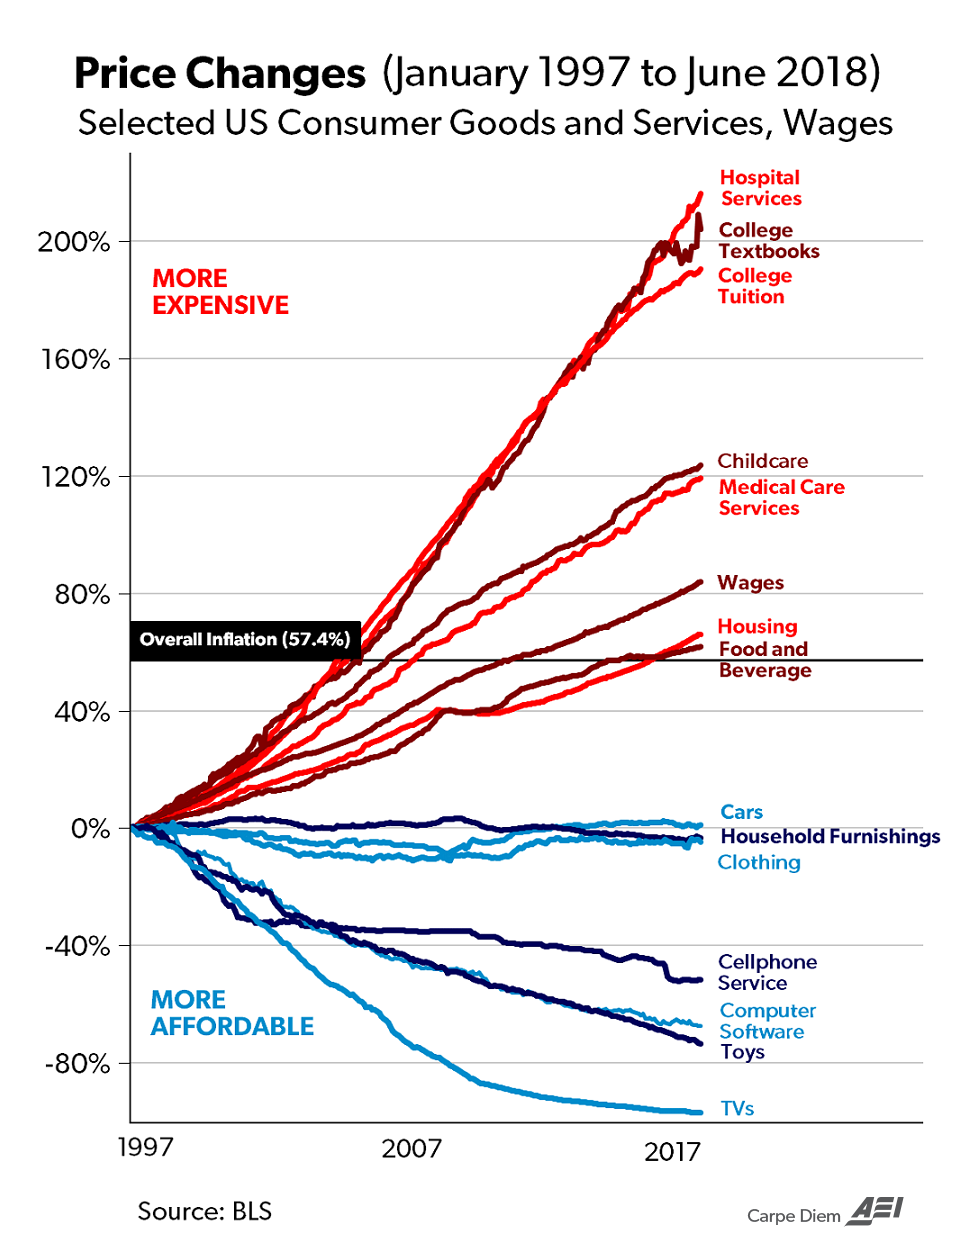
\includegraphics[width=70mm,height=80mm]{cpichart2018a.png}
% \caption{\small From January 1997 to June 2018, the price of college textbooks has increased by approximately 204\%. (source: \alink{aei.org/carpe-diem}{aei.org/carpe-diem}) }\label{fig:cpi-textbooks-2018}
% \end{minipage}
% \hfill
% \begin{minipage}[t]{8.0cm}
% 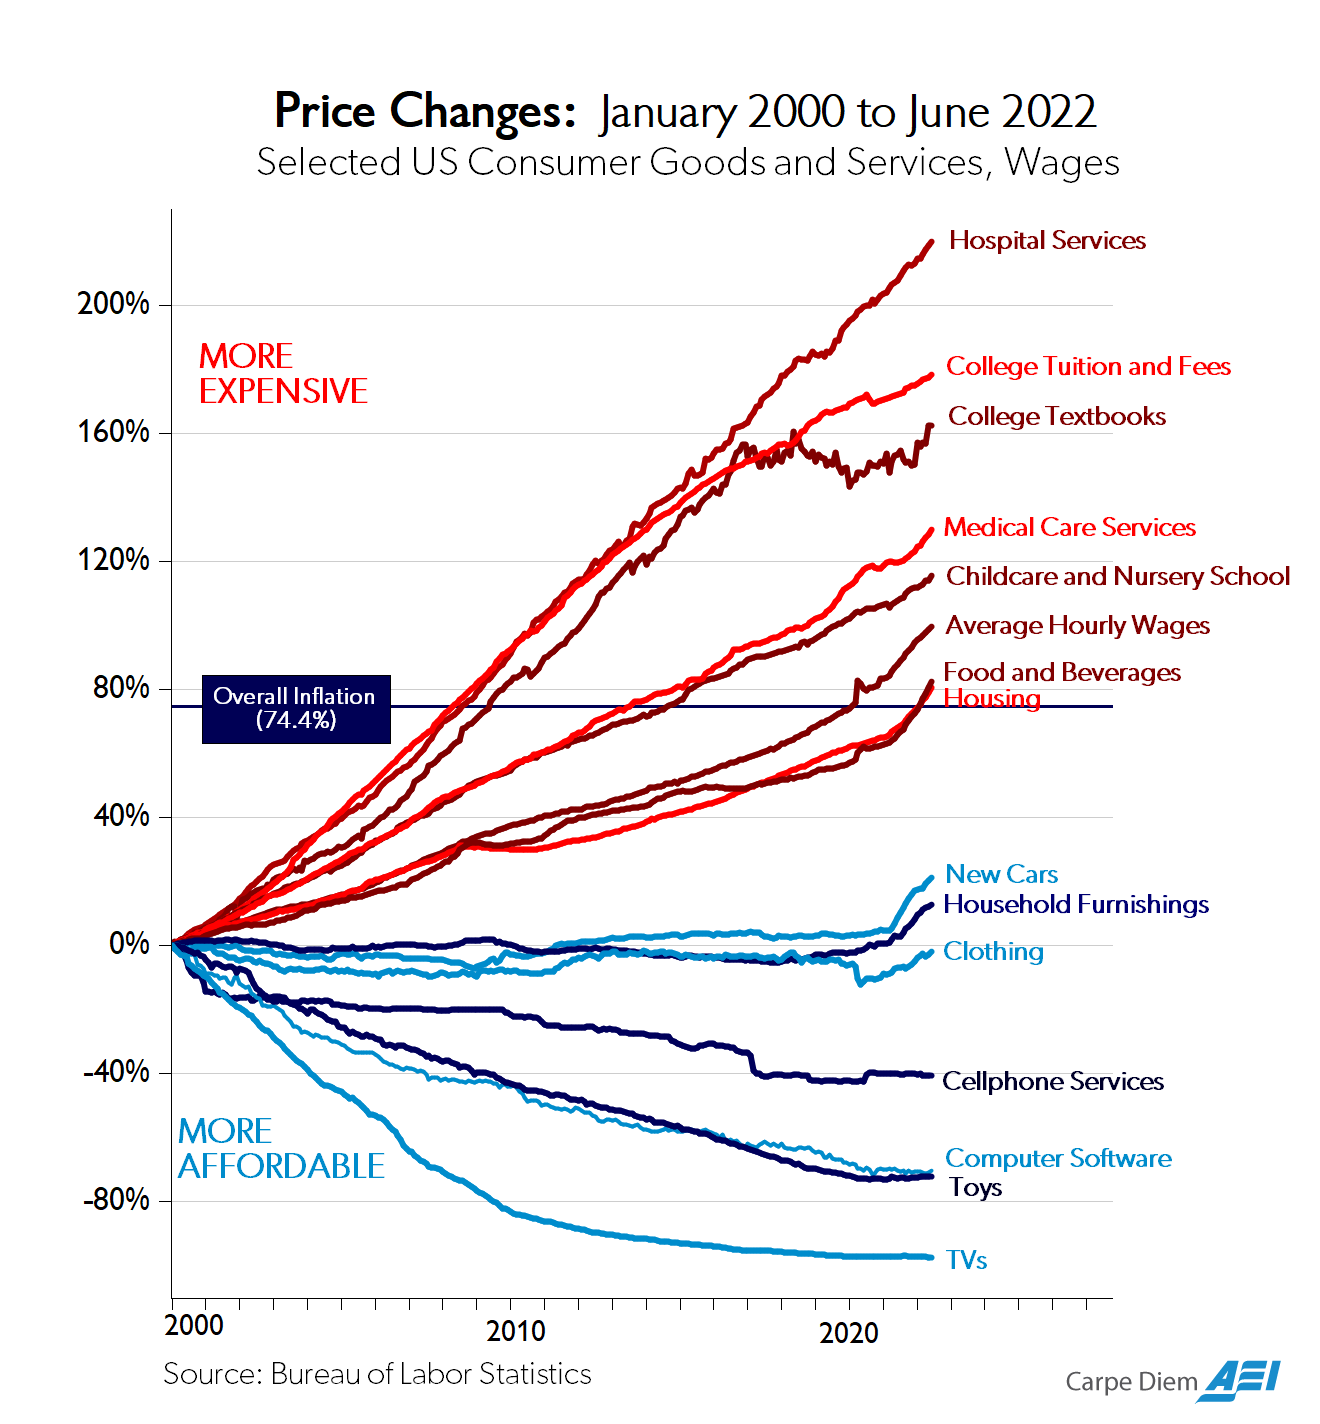
\includegraphics[width=70mm,height=82mm]{cpi2022junea-3.png}
% \caption{\small From January 2000 to June 2022, the price of college textbooks has increased by approximately 162\%. (source: \alink{aei.org/carpe-diem}{aei.org/carpe-diem})}\label{fig:cpi-textbooks-2022}
% \end{minipage}
% \end{figure}

Despite the moderate decrease in college textbook prices in recent years, and the shift by commercial textbook publishers to subscription-based business models, textbook prices remain a substantial burden for students.  In a series of broadly cited annual surveys conducted by the Florida Virtual Campus on students from Florida's public colleges and universities (FLVC)\footnote{Surveys were conducted by FLVC in 2010, 2012, 2016, 2018, and 2022; the 2020 survey was cancelled due to the COVID pandemic.}, more than half (53.5\%) of all 13,000 student respondents in 2022 reported that they had not purchased a required textbook due to its cost \cite{flvc2022}. In the 2018 survey where 22,000 students participated, 66.6\% reported the same.  Other key findings of the 2022 survey found that the high cost of textbooks caused students to:
\begin{compactitem}
\item take fewer courses (43.7\%),
\item not register for a specific course (38.5\%),
\item earn a poor grade due to not being able to afford the textbook (32.4\%), and
\item dropped out of a course (24.2\%).
\end{compactitem}
Students in bachelor degree programs were more likely to spend over \$300 per term on textbooks compared to graduate students or students pursuing an associates degree \cite{flvc2022}.  

While the cost savings for students, educators, and institutions of OER by itself can be an important factor for improved student success and relief for taxpayers \cite{TB-JR-JH:13, RF-RP-BD:15, CW-DD-SC:17}, other benefits of OER include (1) the ability to customize the content to meet the needs of students, (2) the ability to share the content with other educators for improvement, (3) giving students first-day access to course materials which research shows substantially improves learning outcomes \cite{LA:2017}, and (4) giving students the flexibility to engage with the course materials when and where they choose or are able to.  In particular, for students in urban areas that commute to school on public transit, the ability to access course materials on a mobile device is a significant benefit over traditional hard-copy textbooks \cite{CC:17, MS:14}.

\subsection{The Efficacy of OER on Improved Student Outcomes}
Many studies have been performed measuring the efficacy of OER on student performance with mixed results.  Some studies have reported that in some courses, disciplines, or student populations, the adoption of OER results in higher student grades, higher pass rates, lower failing and withdrawal rates, faster progress towards degrees, students taking more courses, and increased engagement and interest in the subject \cite{MC:17, AF-MM:12, KG-WD:17, RG-JM-SW:22, JH-CL:12, JH-LF-DW:16, RJ-FD-RL-KP:18, OO-CH:17, NP-DB:13, RF-RP-BD:15, LF-JH:15, RP:15, TR:15, CB-WC-PH:18}.  One large-scale multi-year study of 21,822 students at the University of Georgia found that the usage of OER had a significant impact on student performance for students with high financial need (specifically, those eligible for a Federal Pell Grant) and for students at greater risk of withdrawing from college such as part-time students \cite{CB-WC-PH:18}.  Of the 5,427 Federal Pell Grant recipients in the study, the number of students in courses adopting OER and those in non-OER courses were approximately evenly split (2,960 in non-OER and 2,467 in OER courses).  The percentage of all Pell recipients receiving a final grade of A or B was 12.7\% higher for students enrolled in courses adopting OER (see Table~\ref{tab:pell-oer}).  Final course grade improvements were also reported for part-time students and non-White students (excluding Asian students) enrolled in OER courses (Tables~\ref{tab:ethnic-oer}-\ref{tab:part-time-oer}).  The DFW rate for Pell recipients and part-time students was 4.43\% and 10.14\%, respectively, lower for students enrolled in courses adopting OER. The study found that course grades increased for all students but DFW rates ``decreased dramaticaly for the student populations we hypothesized would benefit the most from free textbooks''. Overall, the authors of the study noted that ``one would not necessarily anticipate that OER would positively impact the performance of a student who would have otherwise been able to purchase a traditional commercial textbook; however, one would imagine that a free textbook would indeed help those students who might choose to forgo a textbook in a course due to the cost'' \cite{CB-WC-PH:18}.
\begin{table}
\centering
\begin{tabular}{crrrr}
  & \multicolumn{2}{c}{Non-Pell Recipients} & \multicolumn{2}{c}{Pell Recipients} \\ \hline
  \multicolumn{1}{c}{Grade} & \multicolumn{1}{c}{Non-OER} & \multicolumn{1}{c}{OER} & \multicolumn{1}{c}{Non-OER} & \multicolumn{1}{c}{OER}\\ \hline
  A\hspace{1.1ex} & 19.48 & 24.90 & 13.48 & 18.97 \\
  A-\hspace{0.7ex} & 11.72 & 19.83 & 10.17 & 16.66 \\
  B+ & 13.70 & 13.90 & 10.88 & 14.84 \\
  B\hspace{1.1ex} & 22.49 & 16.46 & 20.95 & 18.77 \\
  B-\hspace{0.7ex} & 8.92 & 7.54 & 10.20 & 9.16 \\
  C+ & 6.30 & 3.87 & 8.11 & 4.01 \\
  C\hspace{1.1ex} & 6.88 & 5.20 & 10.30 & 6.65 \\
  C-\hspace{0.8ex} & 0.89 & 0.72 & 1.35 & 0.81 \\
  DFW & 9.62 & 7.57 & 14.56 & 10.13 \\ \hline
\end{tabular}
\caption{Student Grade Distribution Based on Pell Eligibility in non-OER and OER Courses \cite{CB-WC-PH:18}.}
\label{tab:pell-oer}
\end{table}

\begin{table}
\centering
\begin{tabular}{crrrr}
  & \multicolumn{2}{c}{White Students} & \multicolumn{2}{c}{Non-White Students} \\ \hline
  \multicolumn{1}{c}{Grade} & \multicolumn{1}{c}{Non-OER} & \multicolumn{1}{c}{OER} & \multicolumn{1}{c}{Non-OER} & \multicolumn{1}{c}{OER}\\ \hline
  A\hspace{1.1ex} & 20.22 & 26.27 & 11.83 & 15.96 \\
  A-\hspace{0.7ex} & 12.51 & 19.95 & 8.33 & 17.23 \\
  B+ & 13.85 & 14.65 & 10.45 & 13.91 \\
  B\hspace{1.1ex} & 22.42 & 16.05 & 22.08 & 19.52 \\
  B-\hspace{0.7ex} & 8.91 & 7.54 & 10.40 & 8.44 \\
  C+ & 5.96 & 3.24 & 9.27 & 5.47 \\
  C\hspace{1.1ex} & 6.59 & 4.48 & 10.89 & 8.10 \\
  C-\hspace{0.8ex} & 0.85 & 0.62 & 1.48 & 1.22 \\
  DFW & 8.70 & 7.19 & 15.28 & 10.15 \\ \hline
\end{tabular}
\caption{Student Grade Distribution Based on Ethnicity in non-OER and OER Courses \cite{CB-WC-PH:18}}
\label{tab:ethnic-oer}
\end{table}

\begin{table}
\centering
\begin{tabular}{crrrr}
  & \multicolumn{2}{c}{Full-Time Students} & \multicolumn{2}{c}{Part-Time Students} \\ \hline
  \multicolumn{1}{c}{Grade} & \multicolumn{1}{c}{Non-OER} & \multicolumn{1}{c}{OER} & \multicolumn{1}{c}{Non-OER} & \multicolumn{1}{c}{OER}\\ \hline
  A\hspace{1.1ex} & 20.25 & 23.70 & 6.28 & 18.70 \\
  A-\hspace{0.7ex} & 12.67 & 19.47 & 4.45 & 10.98 \\
  B+ & 14.05 & 14.41 & 7.54 & 8.74 \\
  B\hspace{1.1ex} & 22.85 & 17.15 & 18.26 & 14.43 \\
  B-\hspace{0.7ex} & 9.11 & 7.80 & 9.94 & 10.57 \\
  C+ & 6.32 & 3.87 & 9.00 & 4.67 \\
  C\hspace{1.1ex} & 7.48 & 5.49 & 9.11 & 6.71 \\
  C-\hspace{0.8ex} & 0.99 & 0.73 & 1.10 & 1.02 \\
  DFW & 6.28 & 7.38 & 34.33 & 24.19 \\ \hline
\end{tabular}
\caption{Student Grade Distribution Based on Registration Status in non-OER and OER Courses \cite{CB-WC-PH:18}}
\label{tab:part-time-oer}
\end{table}

Other studies have reported no significant differences in student performance in courses adopting OER \cite{VC:18, VC-SK:19, YC-CC:17, RJ-FD-RL-KP:18, ML-OM-CT:08, CL-JL:18, WB-MC-KL:12, JH-DG:13, LF-JH:15, GA-AG-MM:15, OO-CH:17, TR:15, EC:17, CH-SR-GR:17, HR-CH-VM:18, JWS-JP:17} and some studies reported that students enrolled in OER courses performed worse \cite{YC-CC:17, RG:17, TR:15}.  Meta-analyses have been performed to find recurring themes and characteristics in research performed on the efficacy on student learning and perceptions of OER \cite{VC-SK:19, hilton:16, hilton:22}.  Results across the studies analyzed in the meta-analyses \cite{hilton:16, hilton:22} suggests that ``students achieve the same or better learning outcomes when using OER while saving significant amounts of money'' and that ``the results also indicate that the majority of faculty and students who have used OER had a positive experience and would do so again.''  In the meta-analysis \cite{VC-SK:19}, which was based on 22 independent studies, it was concluded that ``there appeared to be no effect on learning performance in courses with open textbooks compared with courses with commercial textbooks'' but that ``there was a significant reduction in the likelihood of students withdrawing from the course'' using OER.  If a student who has fallen behind in a course is able to easily access the required course textbook then it is possible that they are more likely to remain in the course; the most common reason that a student withdraws from a course is that they aniticipate failing the course or receiving a low grade \cite{EW-KB-HK:12}.

\subsection{Barriers to OER Adoption}
Recent studies show that awareness of OER in colleges and universities has grown in the last decade driven primarily by statewide and/or institutional initiatives.  For example, in annual national surveys conducted by Bay View Analytics, which collects for their surveys a representative sample of the broad range of teaching faculty in U.S. higher education, 46\% of polled faculty indicated being aware of both OER and CC licensing in the 2021-2022 survey compared to only 17\% in 2014-2015 \cite{JS-JS:2022}; see Figure~\ref{fig:oer-awareness}.  In the same survey, the majority of respondents indicated that, because of the switch to online learning due to the COVID pandemic, their opinions of online learning improved (54\%) as did their acceptance of digital materials (68\%).  Although progress has been made in increasing college faculty awareness of OER, much work remains to be done to increase the actual usage and creation of quality open educational resources \cite{MB:2022, flvc2022}.
\begin{figure}[t]
\centering
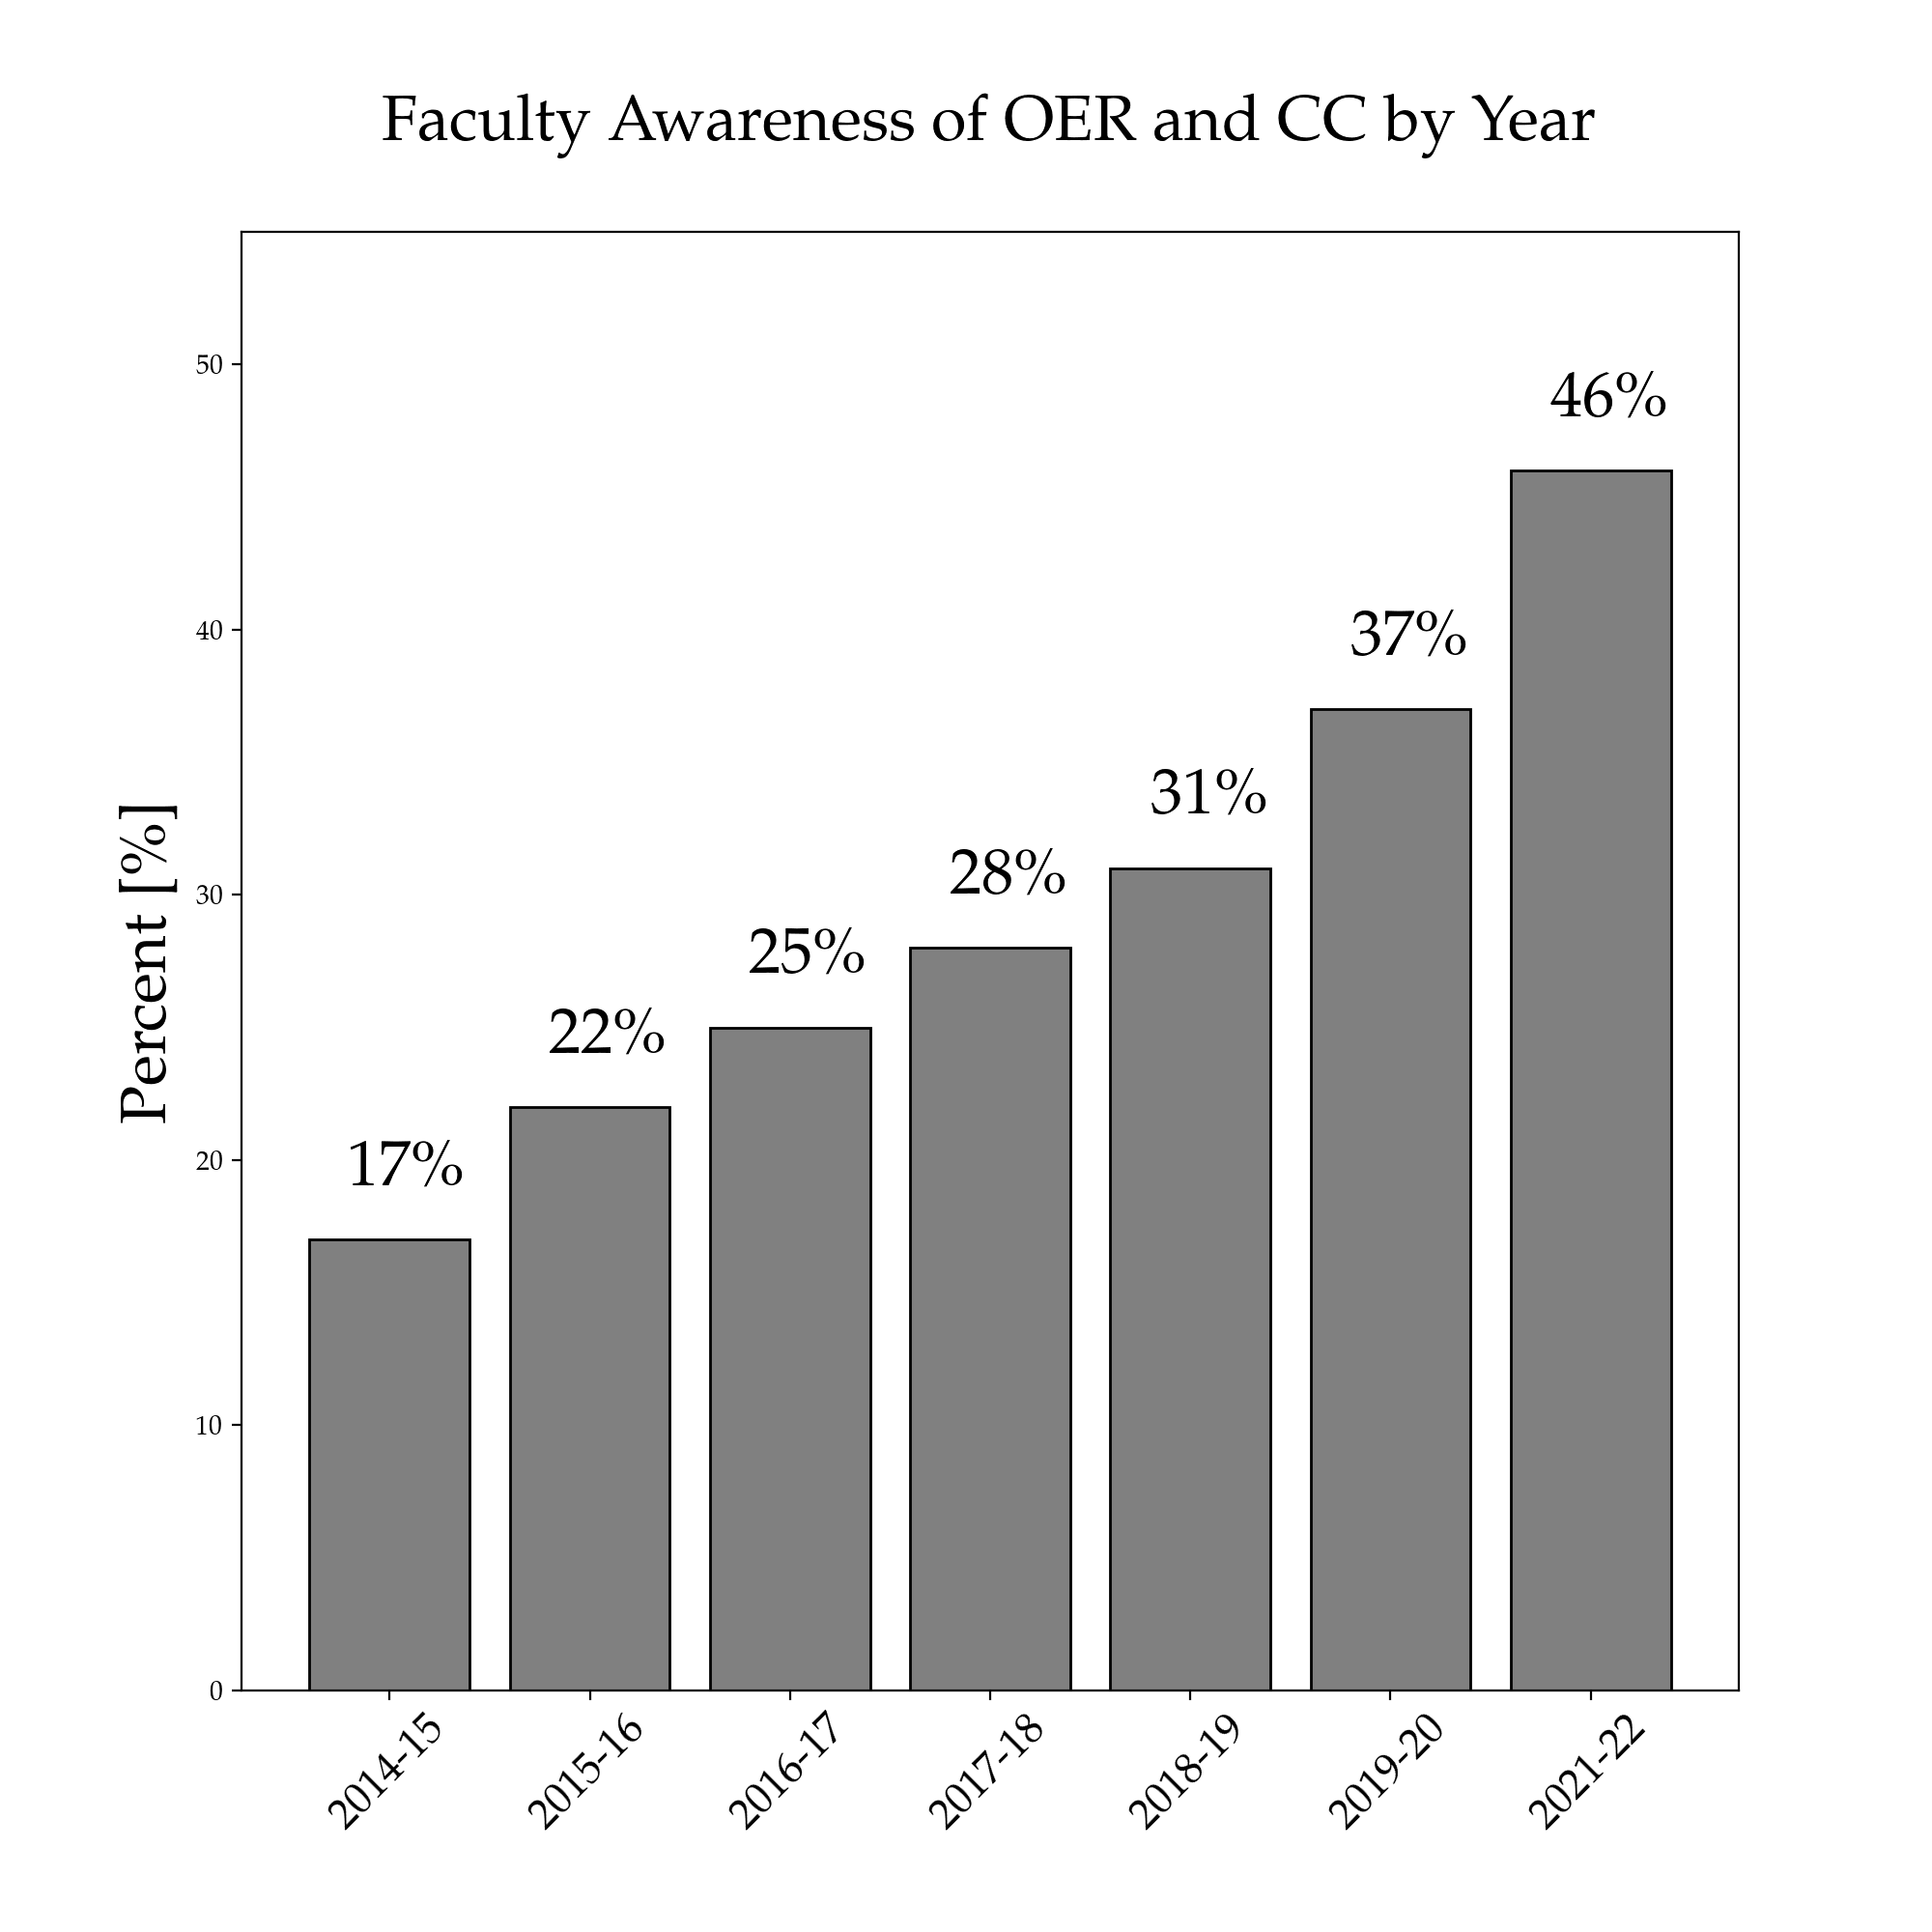
\includegraphics[width=90mm]{oer_awareness.png}
\caption{The percent of U.S. higher education teaching faculty who indicated being aware of both open educational resources (OER) and Creative Commons licenses by year \cite{JS-JS:2022}.}
\label{fig:oer-awareness}
\end{figure}

In communities where OER is adopted, the rights of users to engage in the 5R activities (as described in CC licenses) are often hampered by technological barriers \cite{CC:16, SO:19, MM-EC:19, CE:22}:
\begin{quote}\em
  The truth is that while most open textbooks are legally licensed to be modified, the real-life work involved can sometimes be tough because of technical issues. \cite{CC:16}
\end{quote}
A recent study of open courseware (OCW) on two large OCW platforms (MIT and Delft University of Technology) found that a random sample of ten OCW courses were less open than expected in terms of several factors.  In the study, the openness of OER was evaluated using eight decision factors \cite{MM-EC:19}; one critical factor being the \textbf{file format} used to distribute the content \cite{CE:22}. Of the 10 courses analyzed in the study, all courses were categorized as \textbf{closed} when using the file format as the decision factor to measure openness (see Table~\ref{tab:open-enough}).
\begin{table}
\centering
\renewcommand{\arraystretch}{1.5}
\begin{tabular}{p{5cm}p{5cm}p{5cm}}\hline  
  \rowcolor{Gray}
  \multicolumn{1}{c}{\textbf{Closed}} & \multicolumn{1}{c}{\textbf{Mixed}} & \multicolumn{1}{c}{\textbf{Most Open}}\\ \hline 
A print resource, document image, PDF, or other non-editable format that cannot be altered without expensive software & Editable proprietary file format that could be adapted using open software (e.g. .docx file edited using LibreOffice) & Fully open format (e.g. HTML or .ODF) that could be edited using either open or proprietary software\\[1ex] \hline
\end{tabular}
\caption{The three levels of openness on file format defined as part of the Open Enough framework measuring openness in OER and OCW \cite{MM-EC:19}.}
\label{tab:open-enough}
\end{table}
A principal conclusion made in the study was that OCW were open from a licensing perspective but not well suited for educator adaption which is one of the underlying principles of the OER movement.  In the courses analyzed, the text content of the course was provided almost exclusively in non-editable PDF format.  A similar analysis was performed on the STEM textbooks catalogued by the Open Textbook Library and the results were similar (see Figure~\ref{fig:open-book-formats}); a large portion of the textbooks were available in non-editable format only \cite{CA:22}.  For textbooks containing large amounts of mathematical content, conversion from PDF to other more editable formats is difficult at best or impossible.  From an educators perspective, the use of PDF alone, or other non-editable file format, severely limits or completely eliminates the ability to adapt the material to a local learning environment.
\begin{figure}
  \centering
  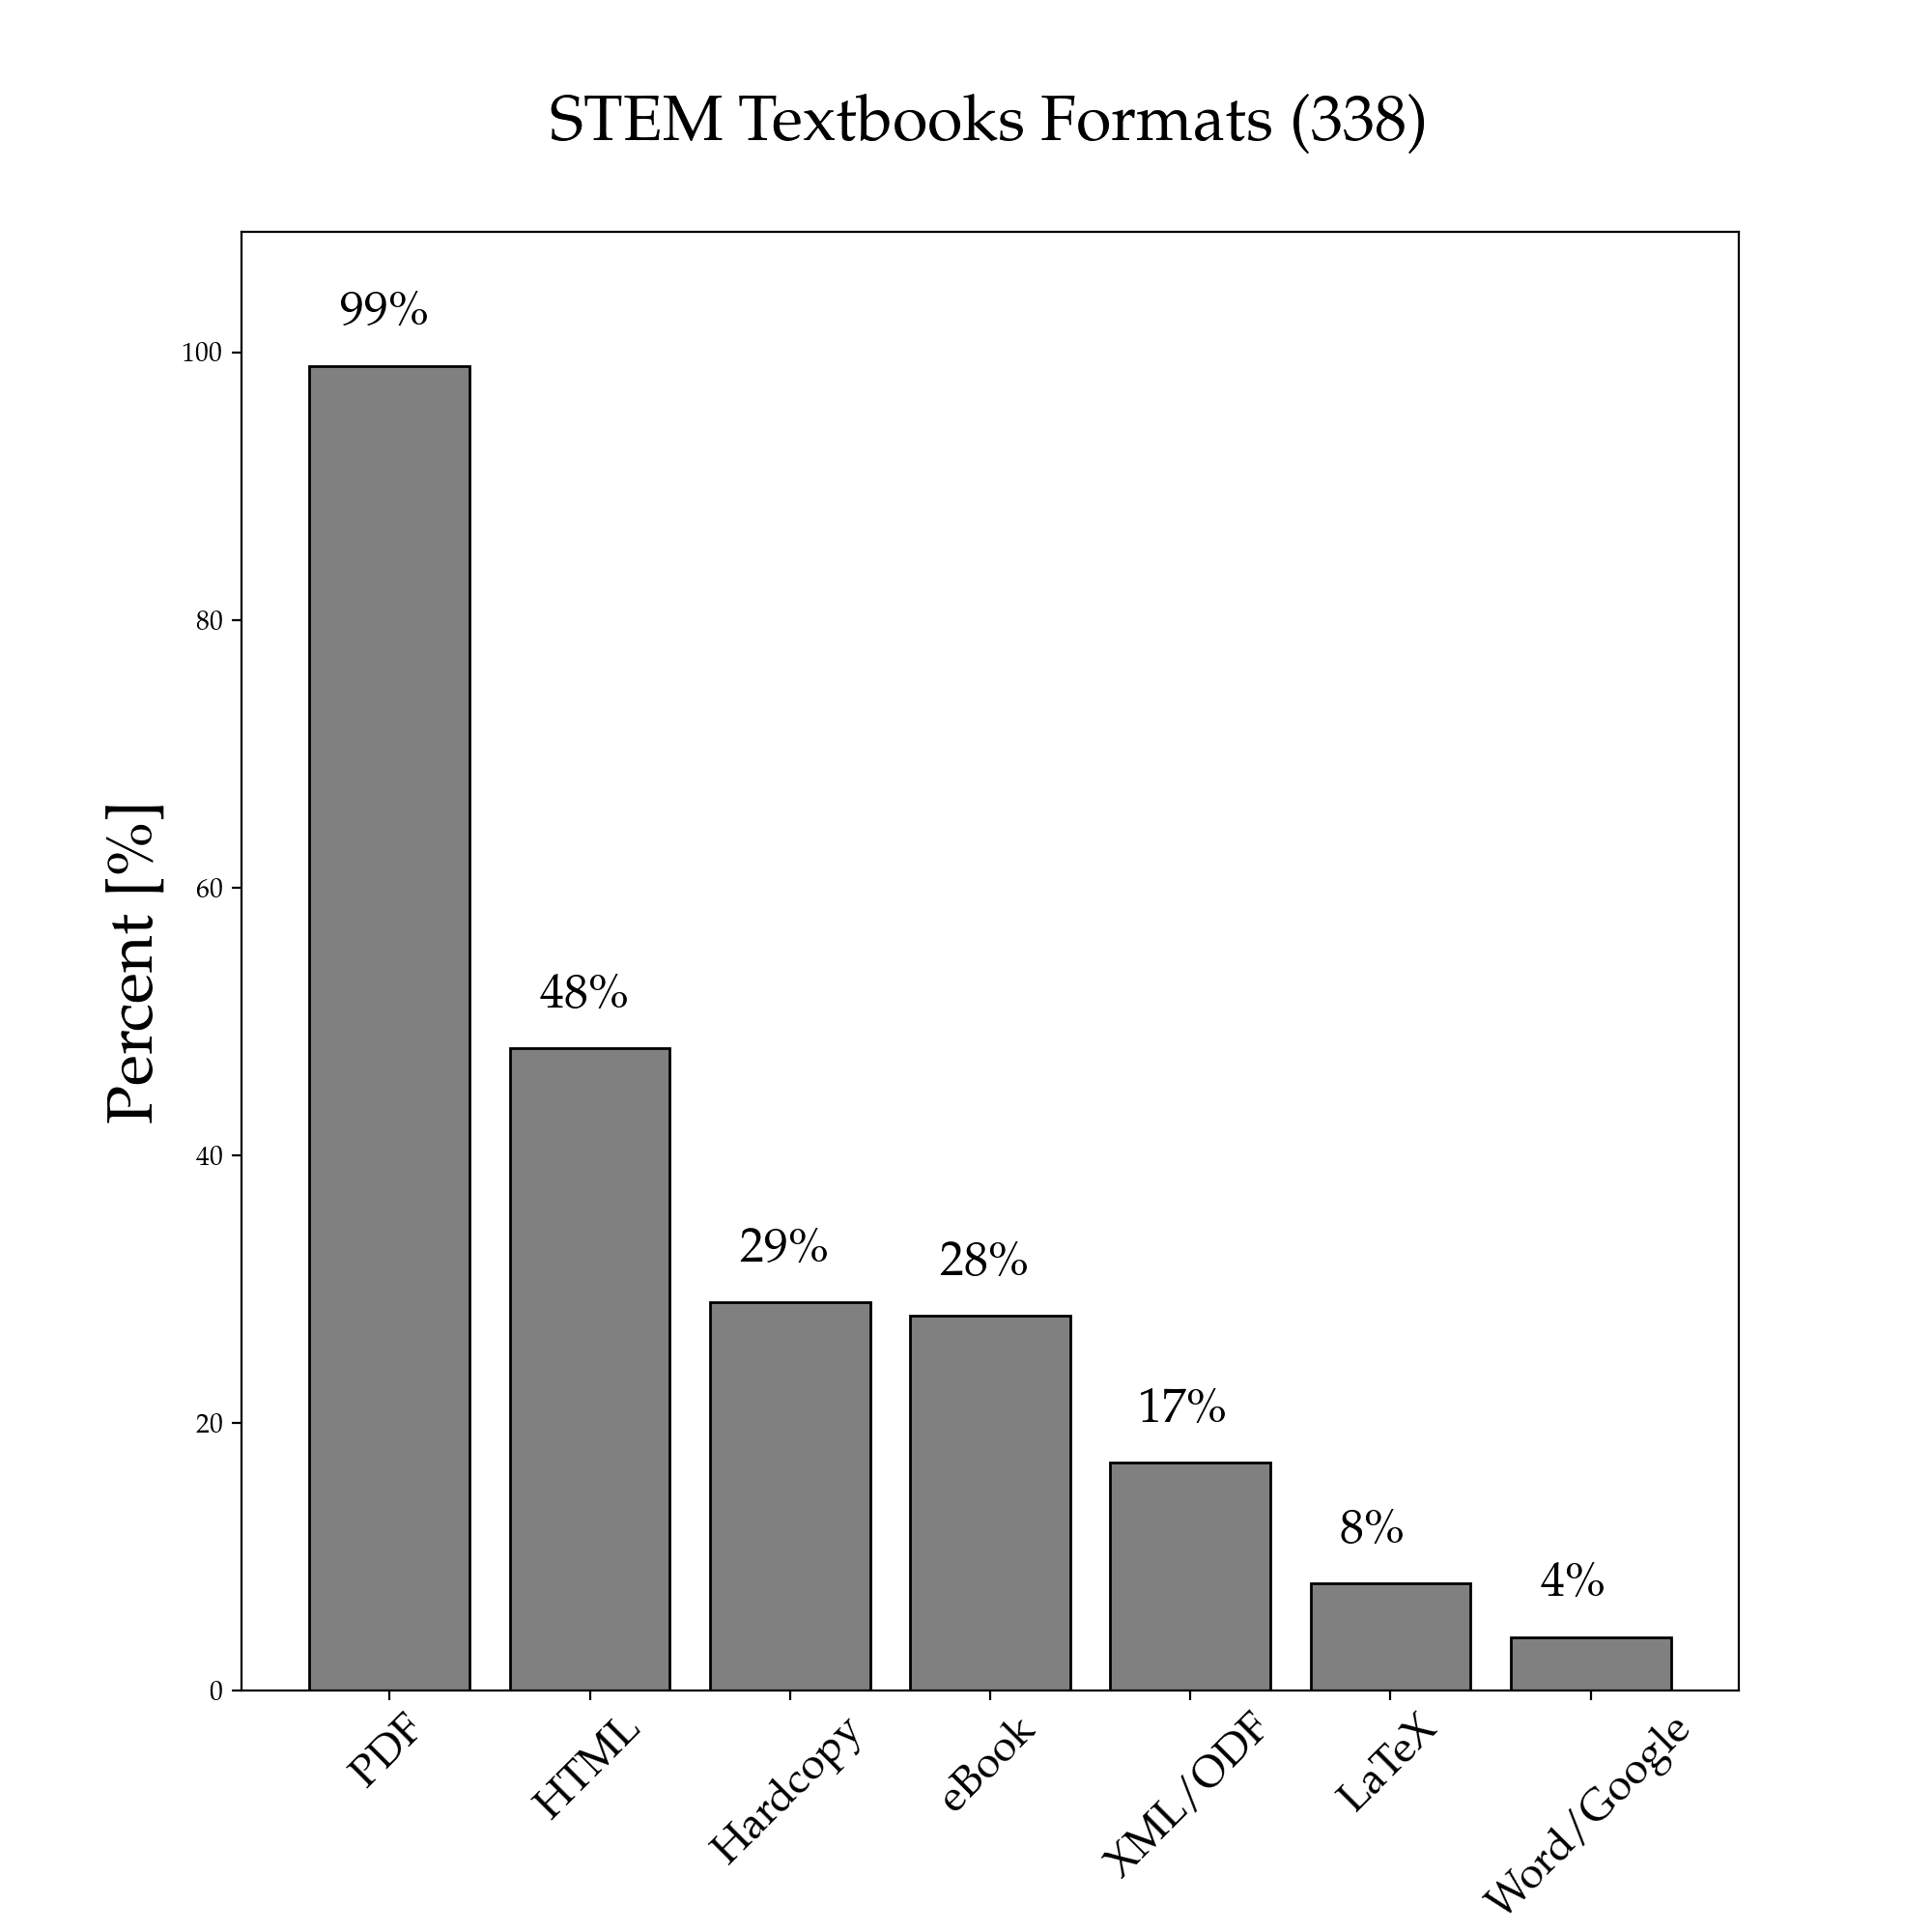
\includegraphics[width=80mm]{stem-textbook-formats.png}
  \caption{On the repository Open Textbook Library, the number of unique textbooks in STEM subjects (Natural Sciences, Computer Science, Engineering, and Mathematics) is 338.  Each textbook is available in at least one format (PDF, HTML, Hardcopy, LaTeX, eBook, MS Word, Google Doc, XML, ODF). Essentially all books are available in PDF (99\%) and nearly half (48\%) are available in HTML.  Data compiled on 12-16-2022 from \alink{open.umn.edu/opentextbooks}{open.umn.edu/opentextbooks}.}
  \label{fig:open-book-formats}
\end{figure}

The file format chosen to distribute OER affects not only the adaptability of course materials but also has implications on the usability of education materials for learners with visual, auditory, or physical disabilities, and in certain situational environments.  According to the W3C Web Accessibility Initiative which develops accessibility standards and guidelines for the web \cite{w3cwai}, ``web accessibility means that websites, tools, and technologies are designed and developed so that people with disabilities can use them'' and that people with disabilities should be able to ``perceive, understand, \textbf{navigate}, and \textbf{interact} with the Web and \textbf{contribute} to the Web''.  However, web accessibility is also important for people without disabilities, for example, for people using the web on small screen sizes such as mobile phones or tablets, for people with slow internet connections or limited bandwidth, or for people in situational environments where lighting and sound are limiting factors to web content consumption.  With regards to educational materials, file formats such as PDF impose significant limitations to interacting with and navigating web content.  According to research performed by the Norman Nielsen Group  web user-experience firm \cite{JN-AK:20}, forcing users to browse PDF files makes usability approximately 300\% worse compared to HTML pages.  Problems with using PDF to deliver and consume content on the web are:
\begin{compactitem}
\item PDF files are optimized for paper sizes, not browser windows or modern screen sizes, 
\item PDF files can be quite large thereby increasing download times when in many cases a user  needs access to only part of the content and not the entire document at once,
\item PDF files are not inherently accessible and can be difficult to navigate especially with small screen sizes or for users with disabilities,
\item PDF files are closed for editing and adaptation without expensive software or technical expertise, and
\item without additional effort by content creators, screen readers cannot reliably parse special elements in a PDF file let alone elements that contain rich mathematical content.
\end{compactitem}
The limitations with using PDF to deliver web content not only affects user experience but also users' perceived \textbf{quality} of the content which studies have shown is a potential barrier to OER adoption by faculty \cite{OB-RB:16, RJ-RP-CH:2016, JS-JS:2018}.

In contrast, HTML is \textit{the} native mark-up language of the web and is the language supported by all web browsers.  HTML is inherently accessible and can be made more accessible with the use of HTML5 semantic tags and special attributes.  Moreover, recent technologies such as MathJax, which has received support from the AMS, SIAM, IEEE, to name only a few, have made it possible to embed mathematical mark-up languages such as LaTeX directly inside HTML documents to create web pages that contain rich mathematical content.  LaTeX is widely used in academia for the distribution and publication of scientific documents, particularly those containing mathematical content.  LaTeX was created in 1985 by Leslie Lamport and is based on the typesetting system TeX created by Donald Knuth in 1978.  LaTeX is widely supported and used by all major publishers of scientific journals and books and is actively developed and maintained by the LaTeX Project.  Many books have been written on the use of LaTeX and is considered the de facto standard for the creation of scientific documents.  Moreover, LaTeX is open-source software and can be easily installed on various computer platforms.

The ability to embed LaTeX in HTML has broad implications on the creation of web-based OER  by mathematicians, computer scientists, engineers, and physicists due to the ubiquitous use of LaTeX in STEM to write course notes, textbooks, and other educational materials.  However, individual content creators and institutional publishers are faced with the difficult and time-consuming task of converting LaTeX source code to HTML in order to take advantage of the native rendering capabilities in web browsers.  Although existing open-source software exist to convert between different mark-up languages such as LaTeX and HTML, most notably \textbf{pandoc}, the conversion process is not always straightforward and requires a certain level of technical expertise.  Alternatively, \textbf{PreTeXt} is a recent mark-up language for authoring and publishing content on the web (and other formats) especially in STEM disciplines but requires authors to learn a new mark-up language and requires the conversion of LaTeX content  to the PreTeXt language.  Although PreTeXt is a promising solution for authoring mathematical content on the web, the ubiquity of LaTeX in STEM fields and the HTML standard built in all web browsers naturally calls for more user friendly and open-source tools to convert between LaTeX and HTML and thereby allows authors to continue to use LaTeX to create STEM educational resources.

\subsection{Open Pedagogy: More Than Just Cost Savings}
Although a main thrust of OER adoption continues to be cost savings, in recent years, advocates of open education have shifted the conversation to the potential improvements to student learning outcomes when faculty decide to exercise the capabilities afforded by open licenses.  As noted by David Wiley, the Chief Academic Officer of Lumen Learning, ``using OER the same way we used commercial textbooks misses the point'' and ``simply adopting open educational resources will not make one's pedagogy magically change to take advantage of the capabilities of the internet" \cite{DW:13}.  A popular sentiment in the open education community is to ``come for the cost savings, stay for the pedagogy''.

Amidst the shift in the open education movement towards the pedagogical benefits of OER, terms such as ``\textbf{open educational practices}'' (OEP), ``\textbf{open pedagogy}'', and ``\textbf{OER-enabled pedagogy}'' have been coined to describe pedagogy that emphasizes a more student-centered approach that empowers students as creators of knowledge and open resources \cite{EM:17, DW:13, DW-JH:18}.  A central idea within this framework is that knowledge consumption and knowledge creation are not separate but rather parallel process that together can help students improve and validate their own learning experiences.  In this OER-enabled teaching paradigm, teachers no longer take the sole responsibility of all-knowing providers of knowledge but instead take on the role of facilitators of knowledge discovery and creation.

In a classroom where open pedagogy is practiced, student assignments are no longer ``disposable''; these are assignments that are ultimately deleted or thrown away by students and that have no value outside of the immediate context in which they were assigned, completed, and graded \cite{DW:13, DW-JH:18}. Many thousands (if not millions) of these assignments are designed and completed each semester requiring large amounts of time and brain power by all involved which can certainly provide valuable opportunities for student learning, open pedagogy advocates call for a shift to using more ``renewable assignments''.

As described in \cite{DW:13, DW-JH:18}, renewable assignments are those that ``support an individual student's learning and result in new or improved open educational resources that provide a lasting benefit to the broader community of learners".  Wiley \cite{DW:13, DW-JH:18} argues that a student who knows that their work might be used by their colleagues or future students to finally help grasp a key difficult concept in the course, or a student who is allowed to have freedom in how to contribute to knowledge creation and thereby pick something they actually enjoy, will engage in the learning process more deeply and thus result in better learning outcomes.

Open pedagogy is the practice of engaging with students as creators of information.  Products of open pedagogy are student-created and openly-licensed so that they may live outside of the classroom in a way that has an impact on the greater community.  Benefits of open pedagogy:
\begin{itemize}
  \item Students' work adding value and provides a sense of agency in their education
  \item Marginalized groups have the potential to be better represented
  \item Reinforces the notion that knowledge is multi-directional
\end{itemize}

Examples of open pedagogy:
\begin{itemize}
  \item Adapt or remix OERs with your students. Even the simple act of adding problem sets or discussion questions to an existing open textbook will help contribute to knowledge, to the quality of available OERs, and to your students' sense of doing work that matters. The adaptation of the open textbook Project Management for Instructional Designers by successive cohorts of graduate students at Brigham Young University provides an excellent example of this approach.
  \item Build OERs with your students. Though students may be beginners with most of the content in your course, they are often more adept than you at understanding what beginning students need in order to understand the material. Asking students to help reframe and re-present course content in new and inventive ways can add valuable OERs to the commons while also allowing for the work that students do in courses to go on to have meaningful impact once the course ends. Consider the examples of the open textbook Environmental Science Bites written by undergraduate students at the Ohio State University or the brief explainer videos created by Psychology students around the world and curated by the NOBA Project.
  \item Build course policies, outcomes, assignments, rubrics, and schedules of work collaboratively with students. Once we involve students in creating or revising OERs or in shaping learning architectures, we can begin to see the syllabus as more of a collaborative document, co-generated at least in part with our students. Can students help craft course policies that would support their learning, that they feel more ownership over? Can they add or revise course learning outcomes in order to ensure the relevancy of the course to their future paths? Can they develop assignments for themselves and/or their classmates, and craft rubrics to accompany them to guide an evaluative process? Can they shape the course schedule according to rhythms that will help maximize their efforts and success?
  \item Teach your students how to edit Wikipedia articles. By adding new content, revising existing content, adding citations, or adding images, students can (with the support of the \alink{https://wikiedu.org/teach-with-wikipedia/}{Wiki Education Foundation}) make direct contributions to one of the most popular public repositories for information.
  \item Let students curate course content. Your course is likely split into a predictable number of units (fourteen, for example) to conform to the academic calendar of the institution within which the course is offered. We would probably all agree that such segmenting of our fields is somewhat arbitrary; there is nothing ontological about Introduction to Psychology being fourteen weeks long (or spanning twenty-eight textbook chapters, etc.). And when we select a novel for a course on postcolonial literature or a lab exercise for Anatomy and Physiology, we are aware that there are a multitude of other good options for each that we could have chosen. We can involve students in the process of curating content for courses, either by offering them limited choices between different texts or by offering them solid time to curate a future unit more or less on their own (or in a group) as a research project. The content of a course may be somewhat prescribed by accreditation or field standards, but within those confines, we can involve students in the curation process, increasing the level of investment they have with the content while helping them acquire a key twenty-first century skill.
  \item Create homework assignments (with solutions), create a study guide for a test, create a practice test, create a mini lesson and present it in class.
  \item Andrew Misseldine from Southern Utah University (https://sites.google.com/a/suu.edu/andrew-misseldine/home) use open pedagogy methods in various courses including abstract algebra, calculus III, and modern geometries.
\end{itemize}

%=========================================================
\section{Project Proposal}

A promise of open educational resources (OER) is that by removing barriers to education such as cost, accessibility, quality, and relevancy to the local learning environment, OER can help improve student outcomes and learning experiences.  A principal belief of OER is that student success can be improved when users of OER can actively participate in the creation and adaptation of educational materials for one's own consumption and for future downstream learners.  Although OER initiatives at global, national, state, and institutional levels have increased awareness of the benefits of OER, the actual practical integration and usage of OER in higher-education is still somewhat limited.  Nonetheless, more and more educators, initially drawn by the cost savings passed on to students by adopting OER, are rethinking their approaches to teaching thanks to the ecosystem surrounding the OER movement and are fostering more student-centered, learner-sourced, community-based, and diversity-infused learning environments.

The goal of this project is to advance undergraduate STEM education by building communities of practice around the creation, usage, improvement, and distribution of open educational resources in undergraduate mathematics courses.  Students at a liberal arts college in varying levels of study and disciplines will engage in learner-sourcing group activities to increase student engagement in the learning process with the aim of solidifying the understanding of learnt material.  Studies have shown that student learning outcomes improve when students are active participants in the creation of learning materials rather than being solely consumers of information.  Students will generate assessments for their peers and simultaneously answer and assess assessments created by their peers. The creation of the assessments will be guided by students' own misconceptions of the content and through self-reflective questioning of perceived understanding and thus also improving the learning experience of future students.  In the process, under-represented students in STEM and future high-school teachers will be trained to use mathematical mark-up languages and version control systems and thereby increasing the number of computer-literate individuals entering the education sector.  A main part of the project will be the development and deployment of a web-based software tool to facilitate the creation of STEM open educational resources with a primary goal of facilitating the reusability of educational materials and increasing the availability of no-cost high-quality resources for instructors and students.  Quantitative and qualitative data will be collected from students to evaluate learning outcomes and perceptions of learner-sourcing activities.  An overarching goal of the project is to implement a model of closer collaboration between educators and students in the creation, delivery, and consumption of STEM education.  Results of the project will be disseminated in national and regional workshops and software tools will be made freely available to the general public.


\subsection{Overview}

%=========================================================
\subsection{Existing Technology}

\subsubsection{MathML}
\textbf{Mathematical Markup Language} (MathML) is a language used to describe the presentation and content of mathematical notation.  MathML is used in web browsers, in computer algebra systems (CAS), print typesetting, and voice synthesis.  The goal of MathML is to enable mathematically rich documents on the web in the same way that HTML has enabled this functionality for text; MathML markup can be written alongside HTML markup.  MathML markup can become quite complicated even for simple mathematical expressions.  As an example, the MathML markup to describe the mathematical expression
\[
x = \frac{-b \pm\sqrt{b^2-4ac}}{2a}
\]
is given by
\begin{verbatim}
    <math>
      <mi>x</mi><mo>=</mo>
      <mfrac>
        <mrow>
          <mo>-</mo><mi>b</mi><mo>&pm;</mo>
          <msqrt>
            <msup><mi>b</mi><mn>2</mn></msup>
            <mo>-</mo><mn>4</mn><mi>a</mi><mi>c</mi>
          </msqrt>
        </mrow>
        <mrow><mn>2</mn><mi>a</mi></mrow>
      </mfrac>
    </math>
\end{verbatim}
whereas the equivalent LaTeX markup is
\begin{verbatim}
    \[
        x = \frac{-b \pm \sqrt{b^2-4ac}}{2a}
    \]
\end{verbatim}
Needless to say, typing MathML by hand can be very tedious and error prone and as such it is not intended to be edited by hand.  Instead, the generation of MathML markup is usually the task of specialized equation editors or the result of a conversion from another markup language such as LaTeX.
 
\subsubsection{LaTeX2HTML}
\textbf{LaTeX2HTML} is a command line utility that converts LaTeX documents to web pages in HTML (latex2html.org).  Documentation for LaTeX2HTML is scarce and not easily accessible for an average computer user.  Basic usage of LaTeX2HTML is not available on the projects website or github page. LaTeX2HTML's conversion of mathematical equations to images to be rendered by the browser is in conflict with the goal of creating mathematically rich documents on the web that are rendered natively by the browser.  Installation of the program requires a more than average level of computer literacy and is not easily accessible to the average computer user.  LaTeX2HTML is not available as a web-based application.

\subsubsection{TeX4ht}
\textbf{TeX4ht} is a command line tool that converts LaTeX documents to various output formats including HTML, ODT (open document format), or DocBook.  According to the programs documentation, modern TeX distributions such as TeX Live and Miktex come with TeX4ht and a related bundling tool called \textbf{make4ht}.  



%=========================================================
\subsection{Placeholder}


%=========================================================
\section{Research Plan and Timeline}


\noindent\textbf{First Year:}  

\noindent\textbf{Second Year:}  

\noindent\textbf{Third Year:}  
%=============================================
\section{Broader Impacts}

\subsection{Research Impact}


%=============================================
\subsection{Training of STEM Students}

\subsection{Educational Impact}    

\section{Results from Prior NSF Support}
The PI has received prior NSF support from the Energy, Power, Control, and Networks program under the Division of Electrical, Communications and Cyber Systems.  The award was granted in 2015 when the PI was a faculty member at California State University Bakersfield (CSUB) (award \#1509966) and was then transferred in 2016 to the PI's current institution SUNY Geneseo (award \#1700578).  The initial award amount was \$231,314 with a start date of September 1, 2015 and end date of November 30, 2016, and the transferred award was in the amount of \$181,889 with a start date of September 29, 2016 and end date of August 31, 2020.  The title of the award was \textit{RUI: Network Structure and Controllability in Natural and Engineered Interacting Dynamic Systems}.

The goal of the research was to advance our scientific understanding of how the local structure of a networked dynamic system influences the global controllability properties of the system and to develop algorithms that avoid undesirable control intervention in such a system. The tools used in the research blended techniques from mathematical control theory, algebraic graph theory, matric analysis, and scientific computing. The results of the research could be used by engineers and scientists to identify control limitations within an existing network and facilitate the construction of new interconnected dynamic systems with specified controllability properties. The PI involved undergraduate students in the research project through focused summer research projects which led to several presentations at national and international conferences by the students.  The results of the research were published in leading mathematics and control engineering journals.

\subsection{Intellectual Merit}
Our research discovered new types of local structures that inhibit the controllability of a network of dynamical system. Previous results in the literature attributed network uncontrollability primarily to local symmetries; our work showed that a much wider class of local structures related to agent clustering can induce uncontrollability and that in most cases these broader structures are present in higher numbers than symmetric structures.

Spectral analysis is closely tied to the controllability properties of a linear control system. Our results provided a rich understanding of the spectral properties of a large class of graphs called \textbf{threshold graphs}. Threshold graphs have received considerable interest in the controls community and by graph theorists because they possess interesting algorithmic properties with regards to the their structure and design. Our spectral results for these graphs can be used to benchmark existing control strategies and in particular, the amount of control energy needed for state transfer and steady--state point stabilization.  Our work also provided a nearly complete characterization of the eigenvalues of a large and rich class of threshold graphs.

The results of the research were published in leading mathematics and control engineering journals and presented at conferences: Automatica, Linear Algebra and Its Applications, IEEE Transactions on Control of Network Systems, the American Control Conference, the Joint Mathematics Meeting, and the MAA Seaway Section meetings.  As of December 30, 2022, our publications have been cited 21 times by publications indexed by MathSciNet and 81 times by publications index by Google Scholar.  Below is the list of publications from our research (student co-authors are indicated by an asterisk):
\begin{enumerate}
\item C.O. Aguilar, B. Gharesifard (2016). On almost equitable partitions and network controllability. {\em Proceedings of the American Control Conference}. pp. 179-184.
\item C.O. Aguilar, B. Gharesifard (2017). Almost equitable partitions and new necessary conditions for network controllability. {\em Automatica}. Vol. 80, pp. 25-31.
\item C.O. Aguilar, J. Lee\myast, E. Piato\myast, B.J. Schweitzer\myast (2018). Spectral characterizations of anti-regular graphs. \textit{Linear Algebra and Its Applications}. Vol. 557, pp. 84-104.
\item C.O. Aguilar (2020). Strongly uncontrollable network topologies. \textit{IEEE Transactions on Control of Network Systems}. Vol. 7, Issue 2, pp. 878-886.
\item C.O. Aguilar, M. Ficarra\myast, N. Schurman\myast, B. Sullivan\myast (2020). The role of the anti-regular graph in the spectral analysis of threshold graphs. \textit{Linear Algebra and Its Applications}. Vol. 588, pp. 210-223.
\end{enumerate}
All of the papers are freely available on the PI's professional academic homepage at SUNY Geneseo.

\subsection{Broader Impacts}
Although a generic or random network will contain no local symmetries or patterns, many real-world networks possess a high-level of symmetry and agent clustering. This is due to the fact that real-world networks grow progressively by adding a new node to the network which introduces tree-like symmetries. When such structures are present in a network, the task of choosing which nodes to control becomes very delicate and in a large network a brute-force approach is infeasible. A specific objective that was obtained in our work was the discovery of a class of networks that were tree-like and have the astonishing property that for no matter what choice of nodes are chosen as control agents, the resulting linear control system is uncontrollable. Such an extreme situation was only thought to occur because of the case of degeneracy in the spectral properties of the underlying system matrix, but the networks we discovered have the property that all eigenvalues of the system matrix are distinct. Although these networks are extremely rare, the properties of these networks provide a rich source of the mechanisms that lead to the uncontrollability of a linear multi-agent system and could provide the seed that leads to a complete characterization of controllability for multi-agent systems.

An important contribution of our research in the wider scientific community is the technique we used to study the eigenvalues of the class of threshold graphs. The class of threshold graph is widely studied due to their numerous applications in resource allocation problems, parallel computing, and psychology. Many algorithmic problems on graphs have been shown to be solved in polynomial time for threshold graphs. Our approach to study threshold graphs used combinatorial matrix methods, eigenvalue interlacing, Toeplitz matrices and Chebyshev polynomials. In particular, using Chebyshev polynomials we were able to give a nearly complete characterization of the eigenvalues of a particular threshold graph which we later proved played a distinguished role among all threshold graphs. Our results on threshold graphs, published in 2019 and 2020, have already been cited 10 times as tracked by MathSciNet. Moreover, we made some conjectures on the eigenvalue distribution of threshold graphs which sparked other researchers in spectral graph theory to contribute to their understanding \cite{MA-EG:23, LA-AE-RB:2017}.

During the award period, 10 undergraduate students were involved in the project, all of which have graduated (9 from SUNY Geneseo and 1 from CSUB). Three of the students involved in the research are pursuing PhD degrees in a STEM field (University of Maryland College Park, Washington University in St. Louis, Syracuse University), and the other 7 are working as software developers and engineers (M\&T Bank, Epic, Corning).  Since SUNY Geneseo is a liberal arts college, we do not offer engineering degrees but nonetheless the students involved in the project have been able to obtain engineering positions both in industry and in graduate school.  Below are some of the accomplishments of the students involved in the project:
\begin{itemize}
\item Seven of the 10 students involved made presentations at national and regional conferences: Joint Math Meeting and the MAA regional meetings. Two of the students presented at the SUNY Geneseo Math Colloquium.
\item After being involved in the project, two of the students were admitted to national REU programs (Michigan State University and James Madison University).
\item Six of the 10 students appear as co-authors in peer-reviewed journal papers.
\item All students learned how to use LaTeX for writing and presenting mathematics, and also learned the programming language Python.
\end{itemize}


During the award period, the PI was invited to host SUNY Geneseo's annual Math Research Weekend (MRW). The Geneseo Research Weekend is a 2-day program where an invited guest leads a team of  undergraduates on a math research topic proposed by the invitee. The MRW is offered to Geneseo students to give them a taste of math research, and sometimes the results are presented at conferences and/or published in a scholarly journal. The invited guest comes to the Geneseo campus and gives a colloquium talk on a Friday afternoon and then Friday evening and all day Saturday works with Geneseo undergraduates on a research topic. The colloquium talk is geared towards a broad audience and also serves to introduce the research topic to the students. The PI chose the topic of Google's PageRank algorithm for the MRW which leveraged the PI's research study on graph theory and spectral analysis in networks.

During the award period, the PI gave two workshops to participants of New York State's Master Teacher Program (SUNY Geneseo region) in 2017 and 2019 on LaTeX and matrix linear algebra, respectively.  The New York State Master Teacher Program is a four-year professional development program for public school K-12 STEM teachers throughout New York state in which participants engage in a minimum of 50 hours of professional development activities each year with the goal of developing knowledge of STEM content, knowledge of pedagogy, and knowledge of students, families, and their communities.

%=============================================
\newpage

% Bibliography
\begin{thebibliography}{99}

  \bibitem{MA-EG:23} Abdi, M., and Ghorbani, E. (2023). Gap sets for the spectra of regular graphs with minimum spectral gap. {\em Discrete Mathematics}. 346(1), 113136.

  \bibitem{CA:22} Aguilar, C.O. (2022). Using file format to measure openness in open educational resources. In preparation.

  \bibitem{LA-AE-RB:2017} Agnihotri, L., Essa, A., \& Baker, R. (2017, March). Impact of student choice of content adoption delay on course outcomes. {\em In Proceedings of the Seventh International Learning Analytics \& Knowledge Conference}. pp. 16-20.

  \bibitem{AA-MA:2021} Alazemi, A., Andelic, M., Koledin, T., and Stanic, Z. (2021). Eigenvalue-free intervals of distance matrices of threshold and chain graphs. {\em Linear and Multilinear Algebra}. 69(16), 2959-2975.

  \bibitem{GA-AG-MM:15} Allen, G., Guzman-Alvarez, A., Molinaro, M., and Larsen, D. (2015). Assessing the impact and efficacy of the open-access ChemWiki textbook project. {\em Educause Learning Initiative Brief}. January 2015.

  \bibitem{MB:2022} Baas, M., van der Rijst, R., Huizinga, T., van den Berg, E., Admiraal, W. (2022). Would you use them? A qualitative study on teachers' assessments of open educational resources in higher education. {\em The Internet and Higher Education}, 54, 100857.

  \bibitem{OB-RB:16} Belikov, O. M., and Bodily, R. (2016). Incentives and barriers to OER adoption: A qualitative analysis of faculty perceptions. Open Praxis, 8(3), 235-246. %DOI: \alink{http://doi.org/10.5944/openpraxis.8.3.308}{http://doi.org/10.5944/openpraxis.8.3.308}
  
  \bibitem{TB-JR-JH:13} Bliss, T., Robinson, T.J., Hilton, J. and Wiley, D.A., 2013. An OER COUP: College Teacher and Student Perceptions of Open Educational Resources. Journal of Interactive Media in Education, 2013(1), p.Art. 4.% DOI: \alink{http://doi.org/10.5334/2013-04}{http://doi.org/10.5334/2013-04}

  \bibitem{WB-MC-KL:12} Bowen, W. G., Chingos, M. M., Lack, K. A., and Nygren, T. I. (2012). Interactive learning online at public universities: Evidence from randomized trials. {\em Ithaka S + R}.

  \bibitem{MC:17} Chiorescu, M. (2017). Exploring open educational resources for college algebra. {\em The International Review of Research in Open and Distributed Learning}, 18(4).

  \bibitem{YC-CC:17} Choi, Y. M., and Carpenter, C. (2017). Evaluating the impact of open educational resources: A case study. {\em portal: Libraries and the Academy}, 17(4), 685-693.

  \bibitem{CC:17} Cooney, C. (2017). What impacts do OER have on students? Students share their experiences with a health psychology OER at New York City College of Technology. {\em International Review of Research in Open and Distributed Learning}, 18(4), 155-178.

  \bibitem{CE:22} Christiansen, E. and McNally, M. (2022). Examining the technological and pedagogical elements of select open courseware. {\em First Monday}. 27, 10.% \alink{https://doi.org/10.5210/fm.v27i10.11639}{https://doi.org/10.5210/fm.v27i10.11639}

  \bibitem{CClicenses:nd} About CC Licenses (n.d.), Creative Commons. (n.d.). Retrieved from \alink{https://creativecommons.org/about/cclicenses/}{https://creativecommons.org/about/cclicenses/}

  \bibitem{VC:18} Clinton, V. (2018). Savings without sacrifice: A case report on open-source textbook adoption. {\em Open Learning}, 33(3), 177-189.

  \bibitem{VC-SK:19} Clinton, V., and Khan, S. (2019). Efficacy of Open Textbook Adoption on Learning Performance and Course Withdrawal Rates: A Meta-Analysis. {\em AERA Open}, 5(3).% DOI: \alink{https://doi.org/10.1177/2332858419872212}{https://doi.org/10.1177/2332858419872212}

\bibitem{CB-WC-PH:18} Colvard, N.\/B., Watson C.\/ E., and Park, H. (2018). The impact of open educational resources on various student success metrics. {\em International Journal of Teaching and Learning in Higher Education, 30(2), 262-276}.

\bibitem{EC:17} Croteau, E. (2017). Measures of student success with textbook transformations: The Affordable Learning Georgia Initiative. {\em Open Praxis}. 9(1), 93-108.

  \bibitem{CC:16} Cuillier, C., Hofer, A., Johnson, A., Labadorf, K., Lauritsen, K., Potter, P., \& Walz, A. (2016). Modifying an open textbook: What you need to know.  {\em Pressbooks}.%  \alink{https://pressbooks.pub/oenmodify/}{https://pressbooks.pub/oenmodify/}

  \bibitem{RF-RP-BD:15} Farrow, R., Pitt, R., de los Arcos, B., Perryman, L.A., Weller, M. and McAndrew, P. (2015). Impact of OER use on teaching and learning: data from OER Research Hub (2013-2014). {\em British Journal of Educational Technology}. 46(5) pp. 972-976.

  \bibitem{unescoforum:02} Forum on the Impact of Open Courseware for Higher Education in Developing Countries, UNESCO, Paris, 1-3 July 2002: final report.  UNESDOC Digital Library.%  \alink{https://unesdoc.unesco.org/ark:/48223/pf0000128515.locale=en}{https://unesdoc.unesco.org/ark:/48223/pf0000128515.locale=en}

  \bibitem{opentextbooksfaq:nd} Frequently Asked Questions (n.d.). Open Textbook Library. Retrieved from \alink{https://open.umn.edu/opentextbooks/faq}{https://open.umn.edu/opentextbooks/faq}

  \bibitem{AF-MM:12} Feldstein, A., Martin, M., Hudson, A., Warren, K., Hilton III, J., and Wiley, D. (2012). Open textbook and increased student access and outcomes. {\em European Journal of Open, Distance, and ELearning}, 15(2).

  \bibitem{LF-JH:15} Fischer, L., Hilton III, J., Robinson, T. J., and Wiley, D.
  A. (2015). A multi-institutional study of the impact of open textbook adoption on the learning outcomes of post-secondary students. {\em Journal of Computing in Higher Education}, 27(3), 159-172.

  \bibitem{flvc2022} Florida Virtual Campus, 2022 Student Textbook and Instructional Materials Survey. Tallahassee, FL. %\alink{https://dlss.flvc.org/colleges-and-universities/research/textbooks}{https://dlss.flvc.org/colleges-and-universities/research/textbooks}.

  \bibitem{KG-WD:17} Grewe, K., and Davis, W. P. (2017). The Impact of Enrollment in an OER Course on Student Learning Outcomes. {\em The International Review of Research in Open and Distributed Learning}, 18(4).

  \bibitem{RG-JM-SW:22} Griffiths, R., Mislevy, J. and Wang, S. (2022). Encouraging impacts of an Open Education Resource Degree Initiative on college students’ progress to degree. {\em Higher Education}. 84, 1089-1106.

  \bibitem{RG:17} Gurung, R. A. (2017). Predicting learning: Comparing an open educational resource and standard textbooks. {\em Scholarship of Teaching and Learning in Psychology}, 3(3), 233-248.

  \bibitem{CH-SR-GR:17} Hendricks, C., Reinsberg, S. A., and Rieger, G. W. (2017). The Adoption of an Open Textbook in a Large Physics Course: An Analysis of Cost, Outcomes, Use, and Perceptions. {\em The International Review of Research in Open and Distributed Learning}, 18(4).

  \bibitem{hilton:16} Hilton J. III. (2016). Open educational resources and college textbook choices: A review of research on efficacy and perceptions. {\em Educational Technology Research and Development}, 64, 573-590.

  \bibitem{JH-LF-DW:16} Hilton, J., Fischer, L., Wiley, D., and Williams, L. (2016). Maintaining momentum toward graduation: OER and the course throughput rate. {\em International Review of Research in Open and Distance Learning}, 17(6), 19-26.

  \bibitem{hilton:22} Hilton, J. (2022). Open educational resources, student efficacy, and user perceptions: a synthesis of research published between 2015 and 2018. {\em Education Tech Research Dev}, 68, 853-876 (2020).% \alink{https://doi.org/10.1007/s11423-019-09700-4}{https://doi.org/10.1007/s11423-019-09700-4}.

  \bibitem{JH-CL:12} Hilton, J., and Laman, C. (2012). One college’s use of an open psychology textbook. {\em Open Learning: The Journal of Open and Distance Learning}, 27(3), 201-217.

  \bibitem{JH-DG:13} Hilton, J., Gaudet, D., Clark, P., Robinson, J., and Wiley, D. (2013). The adoption of open educational resources by one community college math department. {\em The International Review of Research in Open and Distance Learning}, 14(4), 37-50.

  \bibitem{RJ-RP-CH:2016} Jhangiani R., Pitt R., Hendricks C., Key J., Lalonde C. (2016). Exploring faculty use of open educational resources in B.C. post-secondary institutions. {\em BCcampus}. %Retrieved from \alink{https://bccampus.ca/2016/01/27/exploring-faculty-use-of-open-educational-resources-in-b-c-post-secondary-institutions/}{https://bccampus.ca/2016/01/27/exploring-faculty-use-of-open-educational-resources-in-b-c-post-secondary-institutions/}

  \bibitem{RJ-FD-RL-KP:18} Jhangiani, R. S., Dastur, F. N., Le Grand, R., and Penner, K. (2018). As good or better than commercial textbooks: Students' perceptions and outcomes from using open digital and open print textbooks. The Canadian Journal for the Scholarship of Teaching and Learning,9(1), 1-20.

  \bibitem{w3cwai} Introduction to Web Accessibility.  W3C Web Accessibility Initiative. \alink{w3.org}{w3.org}%  Retrieved from \alink{https://www.w3.org/WAI/fundamentals/accessibility-intro/}{https://www.w3.org/WAI/fundamentals/accessibility-intro/}% Accessed on 12-20-2022.

  \bibitem{CL-JL:18} Lawrence, C., and Lester, J. (2018). Evaluating the effectiveness of adopting open educational resources in an introductory American Government course. {\em Journal of Political Science Education}, 14(4), 555-566.

  \bibitem{ML-OM-CT:08} Lovett, M., Meyer, O., and Thille, C. (2008). The Open Learning Initiative: Measuring the effectiveness of the OLI statistics course in accelerating student learning. Journal of Interactive Media in Education, 14, 1-16.

  \bibitem{EM:17} Mays, E.(2017). A guide to making open textbooks with students. The Rebus Community for Open Textbook Creation.

  \bibitem{MM-EC:19} McNally, M. B., and Christiansen, E. G. (2019). Open enough? Eight factors to consider when transitioning from closed to open resources and courses: A conceptual framework. {\em First Monday}, 24(6).% \alink{https://doi.org/10.5210/fm.v24i6.9180}{https://doi.org/10.5210/fm.v24i6.9180}

  \bibitem{oerguidelines} Miao, F., Mishra, S., Orr, D., \& Janssen, B. (2019). Guidelines on the development of open educational resources policies. {\em UNESCO Publishing}.%\newline \alink{https://unesdoc.unesco.org/ark:/48223/pf0000371129}{https://unesdoc.unesco.org/ark:/48223/pf0000371129}

  \bibitem{JN-AK:20} Nielsen, J. and Kaley, A. (2020).  Avoid PDF for On-Screen Reading, {\em Nielsen Norman Group}.% \alink{https://www.nngroup.com/articles/avoid-pdf-for-on-screen-reading/}{https://www.nngroup.com/articles/avoid-pdf-for-on-screen-reading/} Accessed 12-20-2022.
  
  \bibitem{SO:19} Ovadia, S. (2019). Addressing the Technical Challenges of Open Educational Resources.  {\em portal: Libraries and the Academy}, 19(1), 79-93.% \alink{http://doi.org/10.1353/pla.2019.0005}{http://doi.org/10.1353/pla.2019.0005}

  \bibitem{OO-CH:17} Ozdemir, O., and Hendricks, C. (2017). Instructor and student experiences with open textbooks, from the California open online library for education (Cool4Ed). {\em Journal of Computing in Higher Education}, 29(1), 98-113.

  \bibitem{bls} U.S. Bureau of Labor Statistics, {\em Consumer Price Index for All Urban Consumers: College textbooks in U.S. city average}, Series ID CUUR0000SSEA011.% \alink{https://data.bls.gov/cgi-bin/srgate}{https://data.bls.gov/cgi-bin/srgate}

  \bibitem{NP-DB:13} Pawlyshyn, N., Braddlee, D., Casper, L., and Miller, H. (2013). Adopting OER: A case study of crossinstitutional collaboration and innovation. {\em EDUCAUSE Review}.

  \bibitem{perry2018} Perry, M.J. (2018). The CD `chart of the Century' Makes the Rounds at the Federal Reserve. {\em Carpe Diem}.% \alink{https://www.aei.org/carpe-diem/the-chart-of-the-century-makes-the-rounds-at-the-federal-reserve/}{https://www.aei.org/carpe-diem/the-chart-of-the-century-makes-the-rounds-at-the-federal-reserve/}.

  \bibitem{perry2022} Perry, M.J. (2022). Chart of the Day \ldots or Century?. {\em Carpe Diem}.% \alink{https://www.aei.org/carpe-diem/chart-of-the-day-or-century-8/}{https://www.aei.org/carpe-diem/chart-of-the-day-or-century-8/}.

  \bibitem{RP:15} Pitt, R. (2015). Mainstreaming Open Textbooks: Educator Perspectives on the Impact of OpenStax College open textbooks. {\em The International Review of Research in Open and Distributed Learning}, 16(4).

  \bibitem{TR:15} Robinson, T. J. (2015). Open textbooks: The effects of open educational resource adoption on measures of post-secondary student success. Doctoral dissertation. Brigham Young University.

  \bibitem{HR-CH-VM:18} Ross, H., Hendricks, C., and Mowat, V. (2018). Open textbooks in an introductory sociology course in Canada: Student views and completion rates. {\em Open Praxis}, 10(4), 393-403.

  \bibitem{oerworldcongress} Second World OER Congress: Ljubljana OER Action Plan. (2017). UNESCO. \newline Retrieved from \alink{https://unesdoc.unesco.org/ark:/48223/pf0000260762}{https://unesdoc.unesco.org/ark:/48223/pf0000260762}

  \bibitem{JS-JS:2022} Seaman, J.E., Seaman, J. (2022). Turning Point for Digital Curricula: EducationAL Resources in U.S. Higher Education. {\em Bay View Analytics}.% \newline \alink{https://www.bayviewanalytics.com/reports/turningpointdigitalcurricula.pdf}{https://www.bayviewanalytics.com/reports/turningpointdigitalcurricula.pdf}

  \bibitem{JS-JS:2018} Seaman, J.E., Seaman, J. (2002). Freeing the Textbook: Educational Resources in U.S. Higher Education. {\em Bay View Analytics}. %\newline \alink{https://www.bayviewanalytics.com/reports/freeingthetextbook2018.pdf}{https://www.bayviewanalytics.com/reports/freeingthetextbook2018.pdf}

  \bibitem{MS:14} Smale, M.A., \& Regalado, M. (2014). Commuter students using technology. {\em EDUCAUSE Review Online}. Retrieved from \alink{http://www.educause.edu/ero/article/commuter-students-using-technology}{http://www.educause.edu/ero/article/commuter-students-using-technology}  

  \bibitem{CW-DD-SC:17} Watson, C. E., Domizi, D. P., and Clouser, S. A. (2017). Student and Faculty Perceptions of OpenStax in High Enrollment Courses. {\em The International Review of Research in Open and Distributed Learning}, 18(5). %\alink{https://doi.org/10.19173/irrodl.v18i5.2462}{https://doi.org/10.19173/irrodl.v18i5.2462}

  \bibitem{EW-KB-HK:12} Wheland, E.R., Butler, K.A., Karyn, H., Katz, K.B., and Harris, R. (2012). What Are They Thinking? Students' Affective Reasoning and Attitudes about Course Withdrawal. {\em NACADA Journal}. 32(2):17-25.

  \bibitem{wileynd} Wiley, D. (n.d.). Defining the ``open'' in open content and open educational resources.\newline Retrieved from \alink{http://opencontent.org/definition/}{http://opencontent.org/definition/}.

  \bibitem{DW:13} Wiley, D. (2013) What is open pedagogy? \newline Retrieved from \alink{https://opencontent.org/blog/archives/2975}{https://opencontent.org/blog/archives/2975}.

  \bibitem{DW-JH:18} Wiley, D., and Hilton III, J. L. (2018). Defining OER-Enabled Pedagogy. The International Review of Research in Open and Distributed Learning, 19(4).

  \bibitem{JWS-JP:17} Winitzky-Stephens, J. R., and Pickavance, J. (2017). Open educational resources and student course outcomes: A multilevel analysis. {\em The International Review of Research in Open and Distributed Learning}, 18(4), 12.

\end{thebibliography}


\end{document}
